\documentclass[a4paper, 11pt]{article}

\usepackage[utf8]{inputenc}

\usepackage[lmargin=1.5cm,tmargin=2cm,rmargin=1.3cm,bmargin=2cm]{geometry}
\usepackage[onehalfspacing]{setspace}
\usepackage[T1]{fontenc}
\usepackage[brazil]{babel}
\usepackage{float}
\usepackage{polynom}
\usepackage[vlined, portuguese, onelanguage]{algorithm2e}
\usepackage{listings}
\usepackage{xcolor}
\usepackage{titlesec}
\usepackage{verbatim}
\usepackage{circuitikz}
\usepackage{subfigure}

\usepackage{hyperref}
\hypersetup{
    colorlinks = true,
    linkcolor = blue,
    filecolor = magenta,
    urlcolor = cyan,
    citecolor = green,
    pdfpagemode = FullScreen
}

\urlstyle{same}
\usepackage{tikz, pgfplots}
\usetikzlibrary{positioning}

\usepackage{siunitx}
\usepackage[output-decimal-marker={.}]{siunitx}

\usepackage{amsmath,amsthm,amsfonts,amssymb,dsfont,mathtools,blindtext}
\usepackage{cleveref}
\usepackage{graphicx,xcolor,comment,enumerate,multirow,multicol,indentfirst}
\usepackage{graphicx}

\newtheorem{theorem}{Teorema}[section]
\newtheorem{corollary}{Corolário}[theorem]
\newtheorem{definition}{Definição}[section]

\usepackage{stackengine}

\usepackage{lmodern}
%----------------------------------------------------------------------

\pgfplotsset{compat=1.8}

\begin{document}
\section{Binary Logistic Regression}
\begin{center}
        \Large Model
\end{center}

\begin{itemize}
        \item Binary classification: $y\in\{0,1\}$
        \item Want to predict probability of being in a particular class: $P(y = 1|\mathbf{x};\mathbf{w})$
        \item Could fit a linear model: $f(\mathbf{x};\mathbf{w}) = \mathbf{w}^{T}\mathbf{x}$
        \item But this could give predictions outside $[0,1]$ for some test inputs (invalid probabilities)
        \item Use the sigmoid function to force the output to lie in the $[0,1]$ range:\[f(\mathbf{x};\mathbf{w}) = \frac{1}{1 + e^{-\mathbf{w}^{T}\mathbf{x}}}\]
        \item Interpret $f(\mathbf{x}; \mathbf{w}) = P(y = 1|\mathbf{x};\mathbf{w})$, implying $P(y = 0|\mathbf{x};\mathbf{w}) = 1 - f(\mathbf{x};\mathbf{w})$
\end{itemize}

\begin{figure}[H]
        \centering
        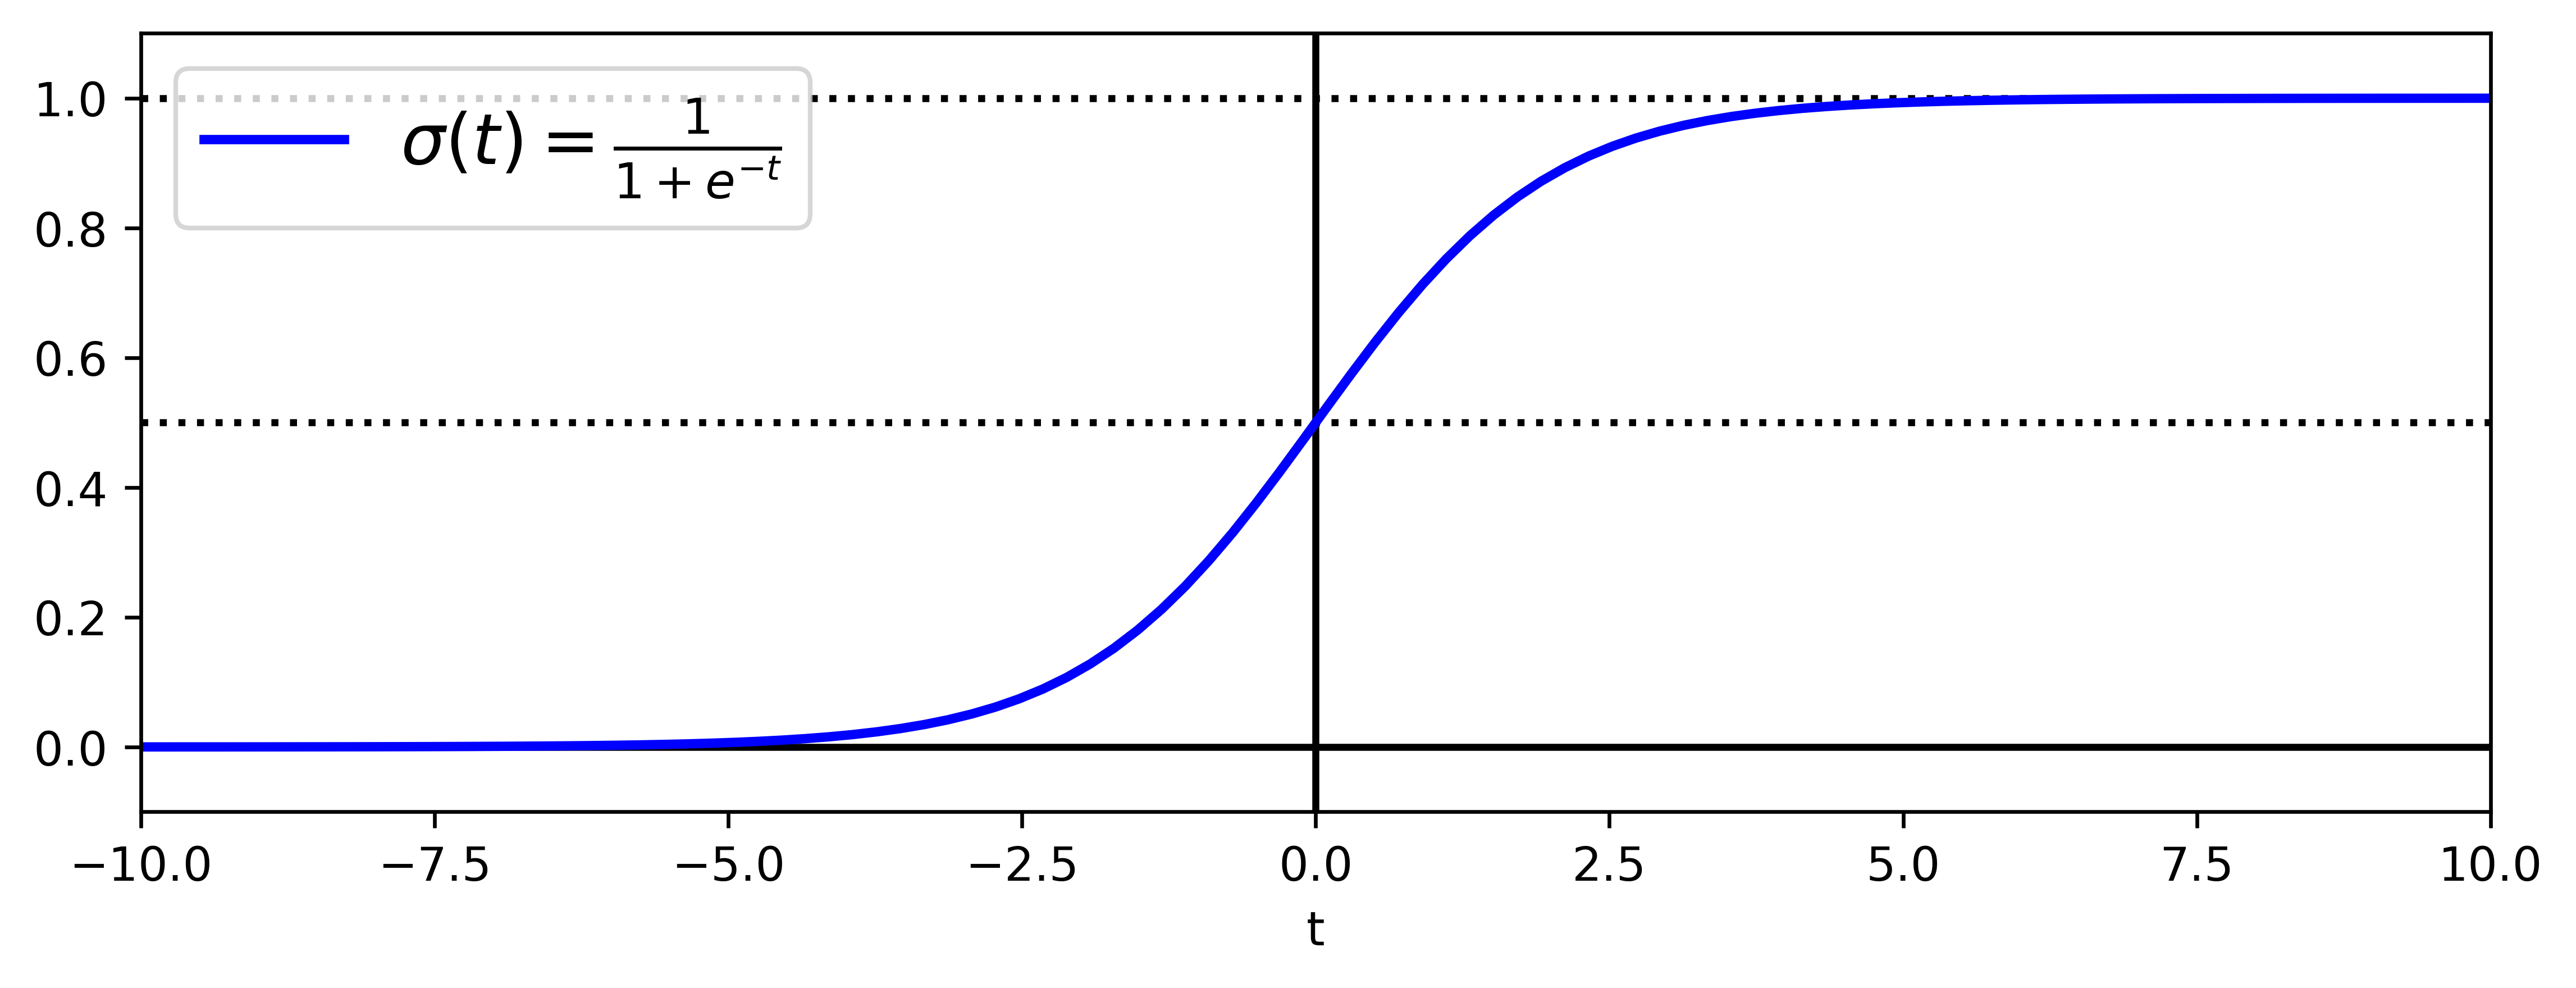
\includegraphics[scale=0.8]{sigmoid.png}
        \caption{Function used to force the output to lie in the $[0,1]$ range}
        \label{fig: Sigmoid Function}
\end{figure}
\newpage
{\Large \textbf{Loss Funciton}}


We observe data $\{(x^{(n)}, y^{(n)})\}_{n = 1}^{N}$, with $y\in\{0, 1\}$, Using maximum likehood:
\begin{align*}
        L(\mathbf{w}) &= P(y^{(1)}|\mathbf{x}^{(1)};\mathbf{w})\cdot P(y^{(2)}|\mathbf{x}^{(2)};\mathbf{w})\cdots P(y^{(n)}|\mathbf{x}^{(n)};\mathbf{w})\\
             &= \prod\limits_{n = 1}^{N}P(y^{(n)}|\mathbf{x}^{(n)};\mathbf{w})
\end{align*}
minimising the negative log likehood
\begin{align*}
        J(\mathbf{w}) &= -\log{L(\mathbf{w})} = -\log{\prod\limits_{n = 1}^{N}P(y^{(n)}|\mathbf{x}^{(n)};\mathbf{w})} = - \sum\limits_{n = 1}^{N}\log{P(y^{(n)}|\mathbf{x}^{(n)};\mathbf{w})}\\
        &(*)\; P(y|\mathbf{x};\mathbf{w}) =\left\{
        \begin{array}{ccc}
                f(\mathbf{x};\mathbf{w}) & if & y = 1\\
                1 - f(\mathbf{x};\mathbf{y}) & if & y = 0
        \end{array}
        \right. = 
        \left\{
        \begin{array}{ccc}
                \sigma(\mathbf{w}^{T};\mathbf{x}) & if & y = 1\\
                1 - \sigma(\mathbf{w}^{T};\mathbf{x}) & if & y = 0
        \end{array}
        \right.\\
        &\implies P(y|\mathbf{x};\mathbf{w}) = \sigma(\mathbf{w}^{T};\mathbf{x})^{y}(1 - \sigma(\mathbf{w}^{T};\mathbf{x}))^{1 - y}\\
        &= -\sum\limits_{n = 1}^{N} \log{[\sigma(\mathbf{w}^{T};\mathbf{x}^{(n)})^{y}(1 - \sigma(\mathbf{w}^{T};\mathbf{x}^{(n)})^{1-y^{(n)}})]}\\
        &= -\sum\limits_{n = 1}^{N} [\log{\sigma(\mathbf{w}^{T};\mathbf{x}^{(n)})^{y}} + (1 - y^{(n)})\cdot\log(1 - \sigma(\mathbf{w}^{T};\mathbf{x}^{(n)}))]
\end{align*}

\subsection{Gradient Descent}
\begin{itemize}
        \item We have some function $J(\mathbf{w})$ that we want to minimise w.r.t parameters $\mathbf{w}$;
        \item Idea: Start with a random $\mathbf{w}$ and then keep updating it to reduce $J(\mathbf{w})$;
        \item This method could get stuck in a local minimum;
        \item As we get closer to the minimum, the step sizes automatically gets smaller.
\end{itemize}
\begin{equation}
        \mathbf{w}_{k + 1} = \mathbf{w}_{k} - \eta_{k}\cdot\frac{\partial J}{\partial\mathbf{w}}
        \label{eq:01}
\end{equation}
\begin{figure}[H]
        \centering
        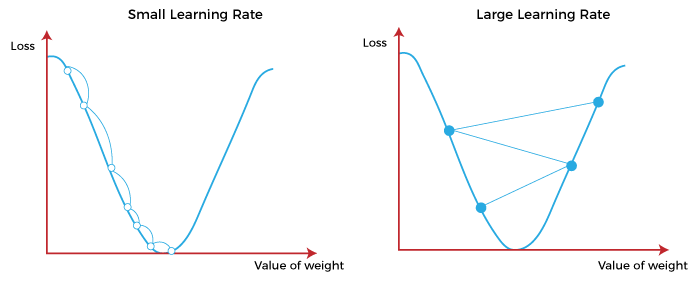
\includegraphics[scale=0.6]{GD_problems.png}
        \label{fig: GD problems}
        \caption{Potential problems}
\end{figure}
\newpage
Returning to Loss Function, we use maximum likehood estimation, or equivalently we want to minimise the negative log likehood:
\begin{equation*}
        J(\mathbf{w}) = -\log{\prod\limits_{n = 1}^{N}P(y^{(n)}|\mathbf{x}^{(n)};\mathbf{w})} = -\sum\limits_{n = 1}^{N} [\log{\sigma(\mathbf{w}^{T};\mathbf{x}^{(n)})^{y}} + (1 - y^{(n)})\cdot\log(1 - \sigma(\mathbf{w}^{T};\mathbf{x}^{(n)}))]
\end{equation*}
To minimise this loss, we need the gradients $\frac{\partial J(\mathbf{w})}{\partial\mathbf{w}}$. Using vector and matrix derivatives, we can show that:
\begin{equation*}
        \frac{\partial J(\mathbf{w})}{\partial\mathbf{w}} = - \sum\limits_{n = 1}^{N}(y^{(n)} - f(\mathbf{x}^{(n)};\mathbf{w}))\mathbf{x}^{(n)}
\end{equation*}
To optimise the loss, you could try setting $\frac{\partial J(\mathbf{w})}{\partial\mathbf{w}} = 0$. But you will see this does not give closed-form solution (as in linear regression). So instead we use gradient descent (\ref{eq:01}).

\begin{figure}[H]
        \centering
        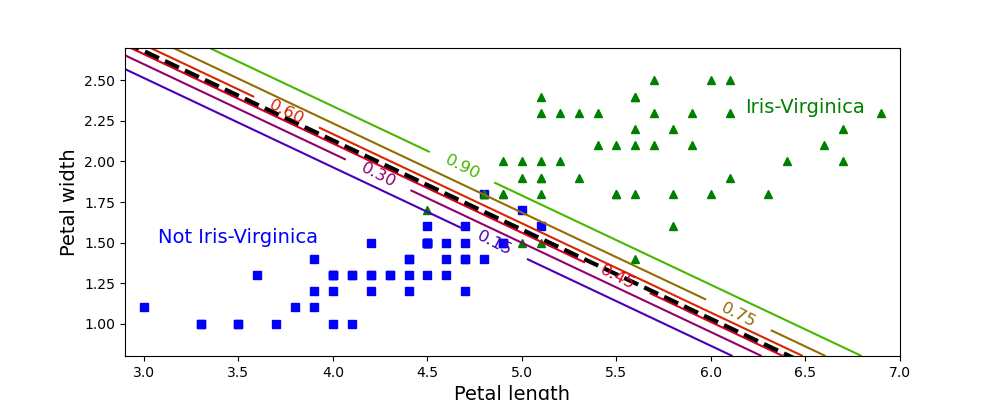
\includegraphics[scale=0.7]{iris.png}
        \caption{Iris-Virginica Prediction in Logistic Regression.}
        \label{fig:Iris}
\end{figure}

\subsection{Decision Boundary}
The decision boundary is the value od $\mathbf{x}$ for which $f(\mathbf{x}; \mathbf{w}) = \sigma(\mathbf{w}^{T}, \mathbf{x}) = 0.5\implies \mathbf{w}^{T}\cdot\mathbf{x} = 0$.
Here it might be easier to explicity include the bias term, i.e. $f(\mathbf{x}; \mathbf{w}) = \sigma(w_0 + \mathbf{w}^{T}\mathbf{x}) = 0.5$. Let's first consisder the 2-D case.
\begin{enumerate}
        \item Sketch the line $w_0 + w_1x_1 + w_2x_2 = 0$ in the $x_1-x_2$ plane;
        \item Sketch the vector $\mathbf{w} = [w_1 w_2]^{T}$ in the same plane;
        \item Redraw the line in $(1)$, but pretend $w_0 = 0$;
        \item Prove that the line in $(3)$ is orthogonal to the line in $(2)$.
\end{enumerate}
This proves that $\mathbf{w}$ is $\perp$ to the decision boundary.

\begin{figure}[H]
        \centering
        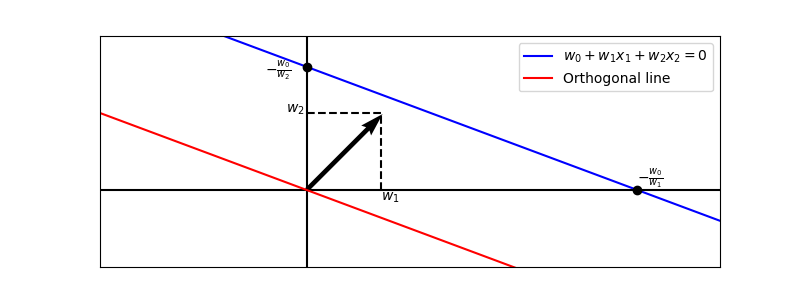
\includegraphics[scale=0.8]{decisionboundary.png}
        \label{fig:DecisionBD}
        \caption{Boundary Decision in 2D}
\end{figure}

we can extend the above to higher dimensions. If we first ignore the bias term, the decision is given by:
\begin{align*}
        w_1x_1 + w_2x_2 + \dots + w_Dx_D &= 0\\
        &=\mathbf{w}^{T}\mathbf{x} = 0
\end{align*}
If we thinck of $\mathbf{w}$ as a vector in $\mathbf{x}$-space, then the $\mathbf{x}$ vectors on the decisions boundary is
orthogonal to $\mathbf{w}$, since their dot product is zero: $\mathbf{w}\cdot\mathbf{x} = 0$. We can add the bias back in:
\begin{equation}
        w_0 + \mathbf{w}^{T}\mathbf{x} = 0
\end{equation}
This has the effect of offshering the decision boundary in $\mathbf{x}$-space.

The lenght of $\mathbf{w}$, i.e. $||\mathbf{w}||$, inlfuences the "steepness" of the decision boundary, for very large $||\mathbf{w}||$, even points that are very
close to the decision boundary will be assigned very high or low probabilities $P(y = 1|\mathbf{x}, \mathbf{w})$, with small $||\mathbf{w}||$, probability assignment will be more graual.

\subsection{Basis function and regularisation}
\textbf{Basis funcitons}:

Anywhere we wrote an $\mathbf{x}$ the features vector $\mathbf{x}$ can be replaced with basis functions $\phi(\mathbf{x})$.

\textbf{Regularization}:

As in linear regression, we can perform regularised logistic regression by penalising the weights:
\begin{align*}
        J(\mathbf{w}) &= -\log{L(\mathbf{w})} + \lambda\sum\limits_{d = 1}^{D}w_{d}^{2}\\
        &= - \sum\limits_{n = 1}^{N}[y^{(n)}\log{\sigma(\mathbf{w}^{T}\mathbf{x}^{(n)})} + (1 - y^{(n)})\log{(1 - \sigma(\mathbf{w}^{T}\mathbf{x}^{(n)}))}] + \lambda\sum\limits_{d = 1}^{D} w_{d}^{2}
\end{align*}

\subsection{Multiclass Logistic Regression}
{\Large\textbf{One-vs-All Classification}}

We define a binary classificator to each class, after that, we attribute a new sample with greater probabilitie.

In this strategy, each classificator is trained using all samples of the training set.


{\Large\textbf{Softmax Regression}}
For binary regression we had $f(\mathbf{w};\mathbf{x}) = \sigma(\mathbf{w}^{T}\mathbf{x}) = \frac{1}{1 + e^{-\mathbf{w}^{T}\mathbf{x}}}$ with $y\in[0, 1]$. We interpreted
the output as $P(y = 1|\mathbf{x};\mathbf{x})$, implying $P(y = 0|\mathbf{x}^{T};\mathbf{w}) = 1 - f(\mathbf{x};\mathbf{w})$.
For the multiclass setting we now have $y\in\{1, 2, \dots, K\}$. Ideia: instead of just outputting a single value for the positive class, let's output a vector
of probabiblities for aech class:
\begin{align*}
        \mathbf{f}(\mathbf{x};\mathbf{W}) = \left[
                \begin{array}{c}
                        P(y = 1|\mathbf{x};\mathbf{W}_1)\\
                        P(y = 2|\mathbf{x};\mathbf{W}_2)\\
                        \vdots\\
                        P(y = K|\mathbf{x};\mathbf{W}_K)
                \end{array}
                \right]
\end{align*}
We will now build up to a model that does this. 



\end{document}
